% !TeX document-id = {babb7a59-8b6e-fdc2-84ad-8d71da78a5e3}
% !TeX TXS-program:compile = pdflatex -synctex=1 -interaction=nonstopmode -output-directory=build -jobname=project-plan_aionfpga_canzani_mueller project-plan.tex
% !TeX TXS-program:bibliography = biber --output-directory build project-plan_aionfpga_canzani_mueller
% !TeX TXS-program:glossary = makeglossaries -d build project-plan_aionfpga_canzani_mueller
% !TeX TXS-program:view = txs:///view-pdf ./build/project-plan_aionfpga_canzani_mueller.pdf

\documentclass[final]{fhnwthesis}

%% Packages
% Main packages
\usepackage[english]{babel}
\usepackage[T1]{fontenc}
\usepackage[utf8]{inputenc}
\usepackage{lmodern}
\usepackage{textcomp}
\usepackage{graphicx}
\usepackage{float}

% Useful packages
\usepackage[pdftex,dvipsnames,table,tables]{xcolor}
\usepackage{csquotes}
\usepackage{siunitx}
\usepackage{xfrac}
\usepackage{listings}
\usepackage{lstautogobble}
\usepackage[bottom]{footmisc}
\usepackage{footnote}
\usepackage{verbatim}
\usepackage[textsize=footnotesize]{todonotes}
%\usepackage{xurl}
%\usepackage{url}
%\usepackage{soul}

% TikZ packages
%\usepackage{standalone}
%\usepackage{tikz}
%\usepackage{circuitikz}
%\usetikzlibrary{arrows}
%\usetikzlibrary{calc}
%\usetikzlibrary{intersections}

% Math packages
\usepackage{amsmath}
%\usepackage{amssymb}
\usepackage{array}
%\usepackage{amsthm}

% Table packages
\usepackage{tabularx}
%\usepackage{longtable}
\usepackage{multirow}
\usepackage{multicol}
\usepackage{booktabs}

% Figure packages
%\usepackage{subfig}
\usepackage{caption}
\usepackage{subcaption}

% PDF packages
\usepackage{pdfpages}
\usepackage{pdflscape}

% Other packages
%\usepackage{xargs}

%% Settings
% Bibliography
\usepackage[style=ieee,dashed=false,urldate=comp,backend=biber]{biblatex}
\addbibresource{literature/bibliography.bib}

% Glossary
\usepackage[toc]{glossaries}
\makeglossaries

\newglossaryentry{test}
{
    name=Test,
    description={Just a test}
}


% Graphics
\graphicspath{{./graphics/}}

% Listings
% purple {0.776,0.584,0.776} / yellow {0.976,0.682,0.341} / orange {0.976,0.482,0.341}
\definecolor{keywordcolor}{rgb}{0.925,0.376,0.4} % red
\definecolor{commentcolor}{rgb}{0.651,0.675,0.725} % gray
\definecolor{stringcolor}{rgb}{0.6,0.78,0.58} % green
\definecolor{backgroundcolor}{rgb}{0.976, 0.98, 0.98} % light gray

\lstdefinestyle{C++}{
    autogobble,
    backgroundcolor=\color{backgroundcolor},
    commentstyle=\color{commentcolor},
    keywordstyle=\color{keywordcolor},
    numberstyle=\tiny\color{commentcolor},
    stringstyle=\color{stringcolor},
    basicstyle=\ttfamily\footnotesize,
    breakatwhitespace=false,
    breaklines=true,
    breakautoindent=true,
    breakindent=50pt,
    escapeinside={(*}{*)},
    captionpos=b,
    keepspaces=true,
    numbers=left,
    numbersep=5pt,
    showtabs=false,
    showspaces=false,
    showstringspaces=false,
    tabsize=2,
    language=C++
}


% Other
%\geometry{twoside=false}
\setlength{\marginparwidth}{2cm}
\overfullrule=5em

%% Custom definitions
% Table definitions
\newcolumntype{L}[1]{>{\raggedright\arraybackslash}p{#1}}
\newcolumntype{C}[1]{>{\centering\arraybackslash}p{#1}}
\newcolumntype{R}[1]{>{\raggedleft\arraybackslash}p{#1}}
\newcolumntype{M}[1]{>{\centering\arraybackslash}m{#1}}
\newcolumntype{N}{@{}m{0pt}@{}}

% Month
\newcommand{\MONTH}{
	\ifcase\the\month
	\or January
	\or February
	\or March
	\or April
	\or May
	\or June
	\or July
	\or August
	\or September
	\or October
	\or November
	\or December
	\fi}

% URL
\urlstyle{same}

% siunitx
\sisetup{per=fraction}



\title{\textbf{{\Huge AI High-Performance Solution \\[2mm] on FPGA}}}
\author{\textit{{\LARGE Project Plan}}}
\date{}

\begin{document}

% Title page
\selectlanguage{english}
\pagenumbering{gobble}
\maketitle

\begin{figure}[H]
  \centering
  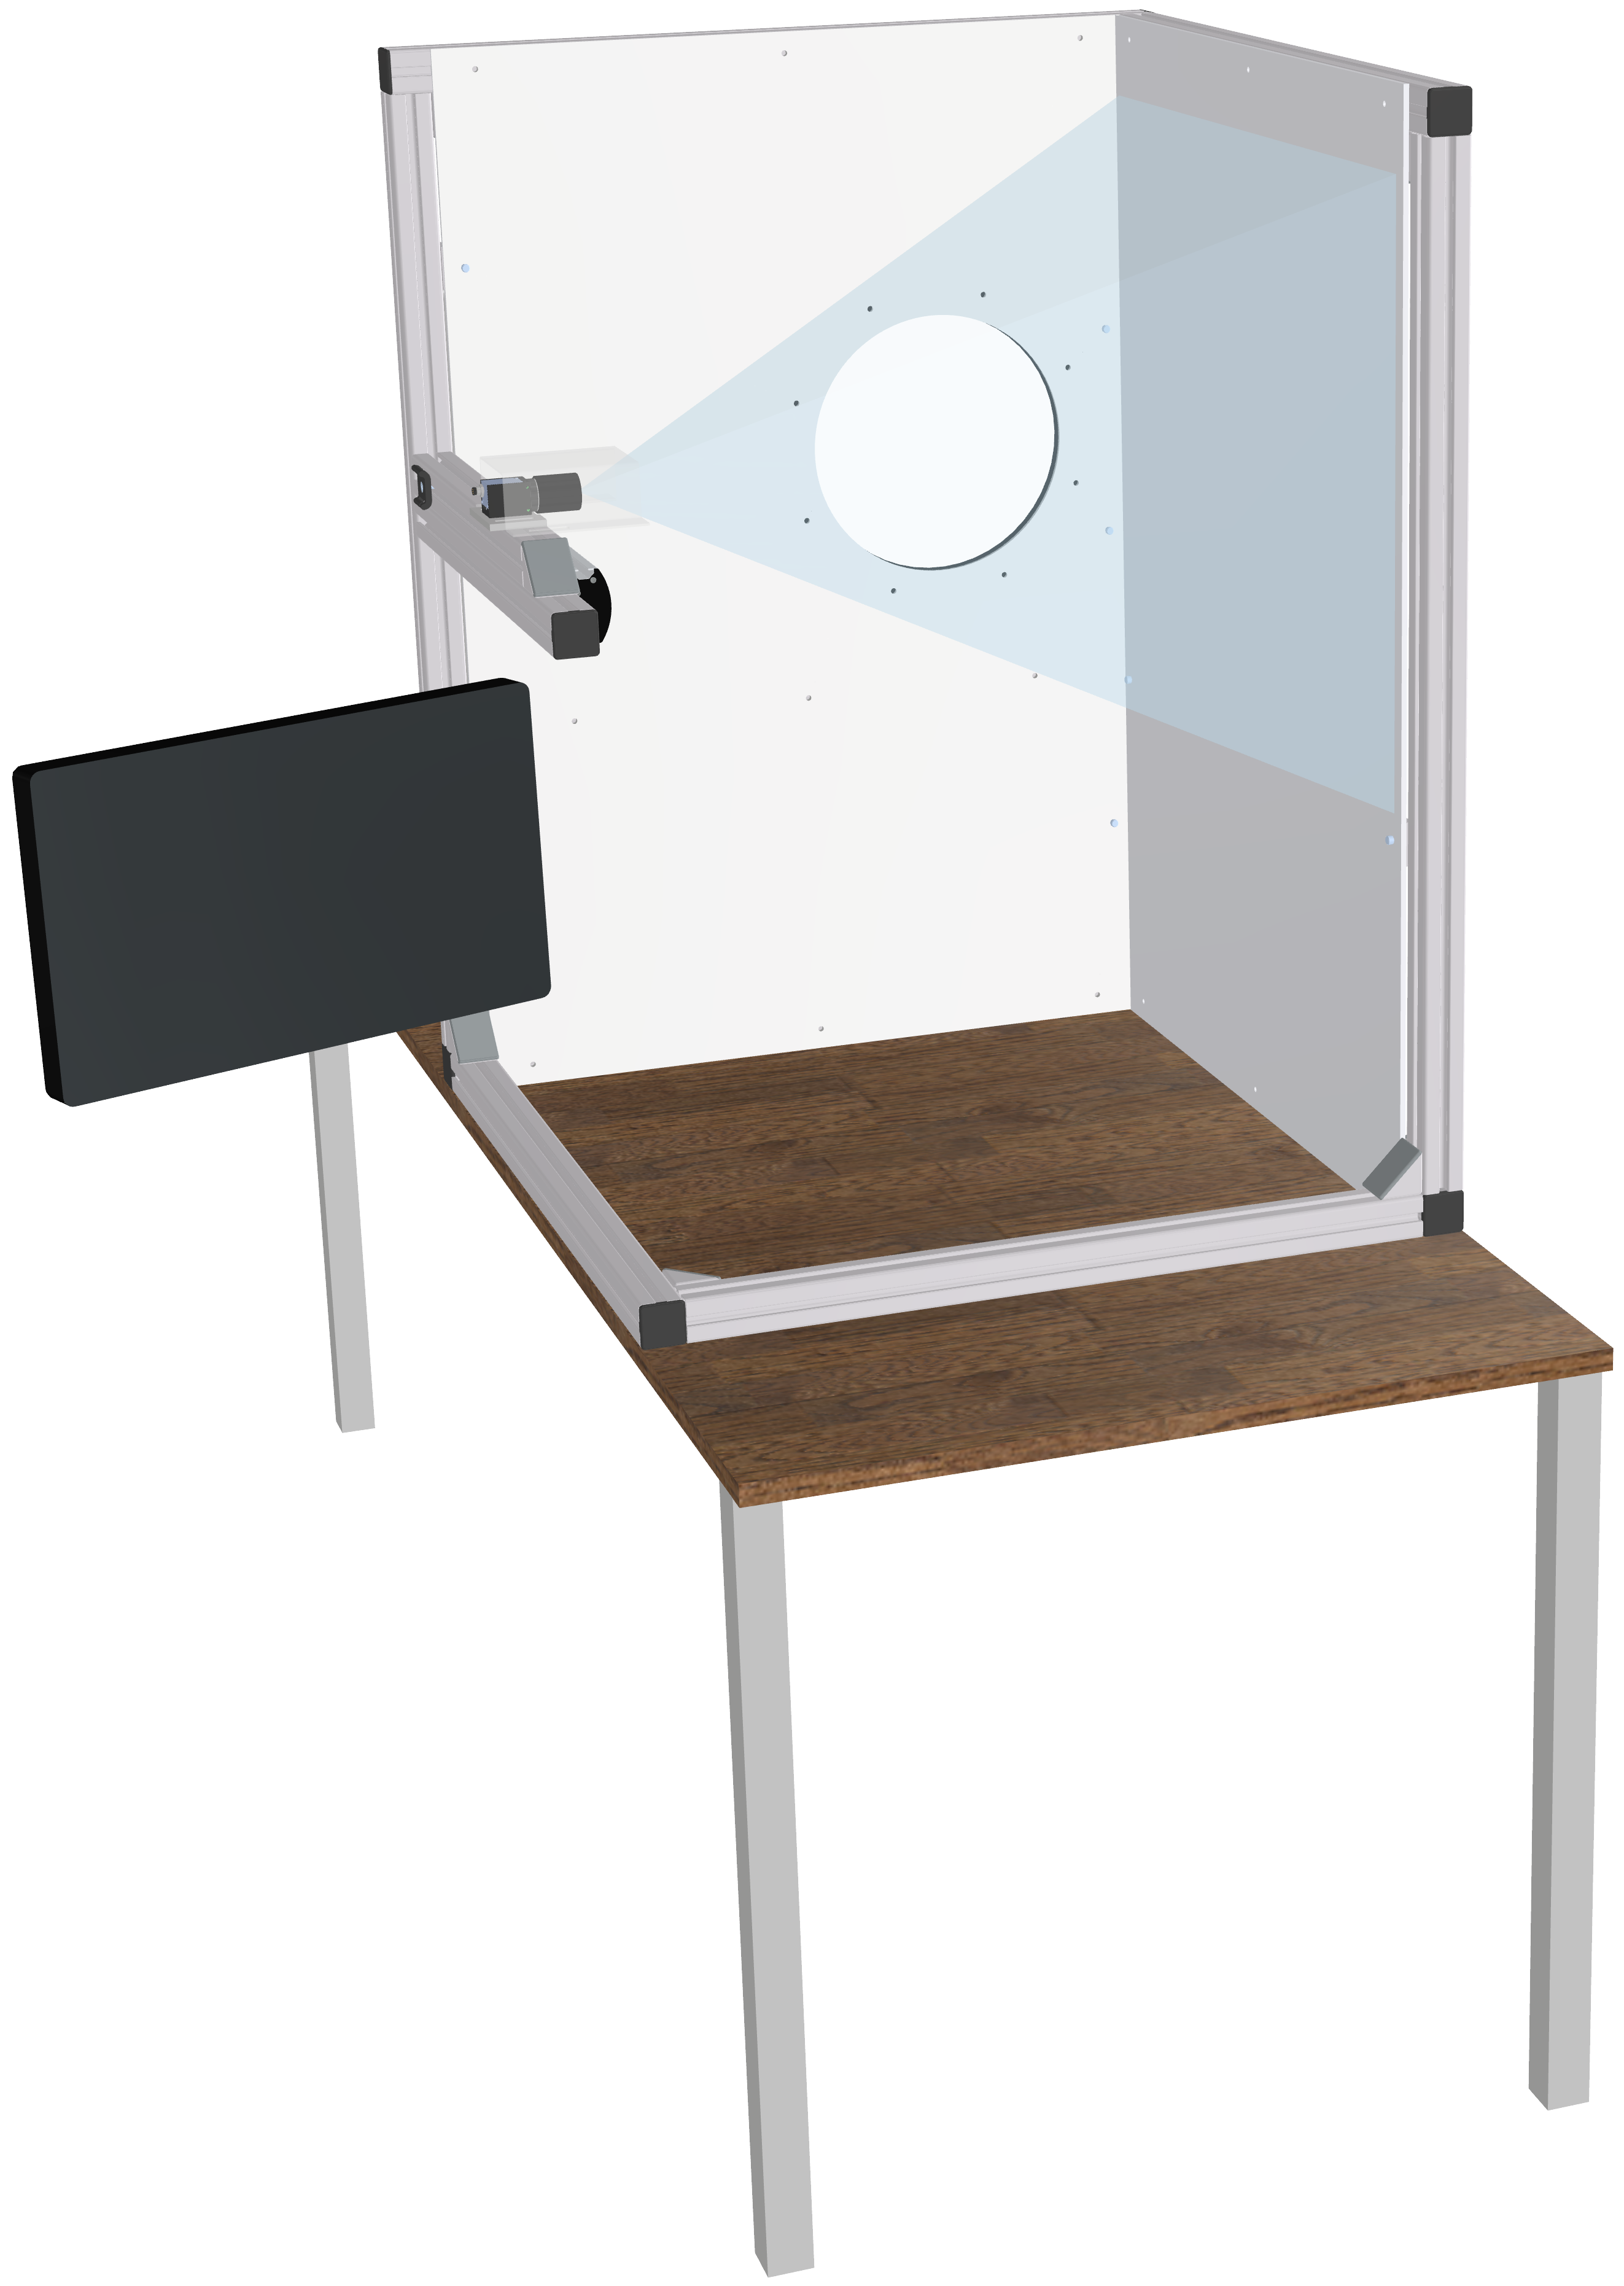
\includegraphics[width=0.55\textwidth]{top_assembly}
\end{figure}

\vfill
\begin{center}
  \begin{tabular}{>{\bfseries\large}rl}
    Degree Program & Electrical Engineering and Information Technology \\[2mm]
    Customer       & Institute for Sensors and Electronics \\[2mm]
    Coaches        & Prof. Michael Pichler, Prof. Dr. Hanspeter Schmid \\[2mm]
    Expert         & Dr. J\"urg M. Stettbacher \\[2mm]
    Team           & Nico Canzani, Dominik M\"uller \\[2mm]
    Date           & \today
  \end{tabular}
\end{center}
\clearpage

% Contents
\pagenumbering{roman}
\tableofcontents
\clearpage

% Sections
\pagenumbering{arabic}
% general goal of the project
% what was done in the past project
% what needs to be done

\chapter{Initial Situation}
\label{ch:initial_situation}


\chapter{Project Goal}
\label{ch:project_goal}

The goal of this project is to develop and train a CNN model and implement it on an FPGA development board.
Images of the throwing objects can then be captured by the camera, classified on the FPGA and displayed on the monitor.

The respective objectives for this project are specified in the following table:\\

\begin{tabularx}{\textwidth}{L{3.05cm}X}
  \toprule
  \textbf{Objective} & \textbf{Description} \\
  \midrule
  CNN Model & A CNN model is developed and trained on a computer. This is done in Python 3 using TensorFlow 2 and the previously collected dataset. \\
  \midrule
  High-Performance Implementation & The advantages of an FPGA flow into the development. Thus, special attention is paid to the performance of the system. \\
  \midrule
  Display & A monitor displays the image of the object that was thrown. Furthermore, the best guess of the CNN as well as additional statistics are shown. \\
  \midrule
  Verification & The accuracy and performance of the CNN model implemented on the FPGA is verified. These results are compared to the computer results. \\
  \bottomrule
\end{tabularx}

\chapter{Deliverables}
\label{ch:deliverables}

The following table lists all deliverables with their respective deadlines:\\

\begin{tabularx}{\textwidth}{Xl}
  \toprule
  \textbf{Deliverable} & \textbf{Deadline} \\
  \midrule
  Project Plan & March 06, 2020 \\
  Demonstrator & August 14, 2020 \\
  Working Repository & August 14, 2020 \\
  Bachelor Thesis incl. Developer Guide & August 14, 2020 \\
  Poster & August 14, 2020 \\
  Thesis Defense & September 10/11, 2020 \\
  Fact Sheet & September 19, 2020 \\
  \bottomrule
\end{tabularx}

\chapter{Concept}
\label{ch:concept}

This chapter briefly explains the concept of this project.
The three main parts are the demonstrator, the training and the inference.

\section{Demonstrator}
\label{sec:demonstrator}

The demonstrator --- a throwing booth --- was not entirely finished during the previous project.
However, the things that still need to be done are not that time-consuming.
For this reason, those tasks are not included in the timetable.
They are carried out on the side to fill time gaps (e.g. during the training of a CNN model).

\section{Training}
\label{sec:training}

The development and training of the CNN model is an iterative process.
Various CNN architectures are experimented with and the results are compared to each other.
Furthermore, the labeled dataset allows for some experimentation as well.
For instance, each image has a label that indicates whether the object was fully or only partially visible.

\section{Inference}
\label{sec:inference}

A high-performance solution requires fast image acquisition and low-latency inference.
To implement the necessary components on the MPSoC with the integrated FPGA, a variety of toolchains and Linux-based operating systems can be used.
These options are initially examined carefully in order to select the most suitable one.

The specific implementation of the image acquisition and the inference depends on the overall performance and the available resources of the MPSoC development board.
For this reason, several performance tests are carried out to evaluate its real-time capabilities.

The final step is to verify the performance and accuracy of the entire system.
The accuracy is additionally compared to the accuracy of the computer solution.

\chapter{Timetable}
\label{ch:timetable}
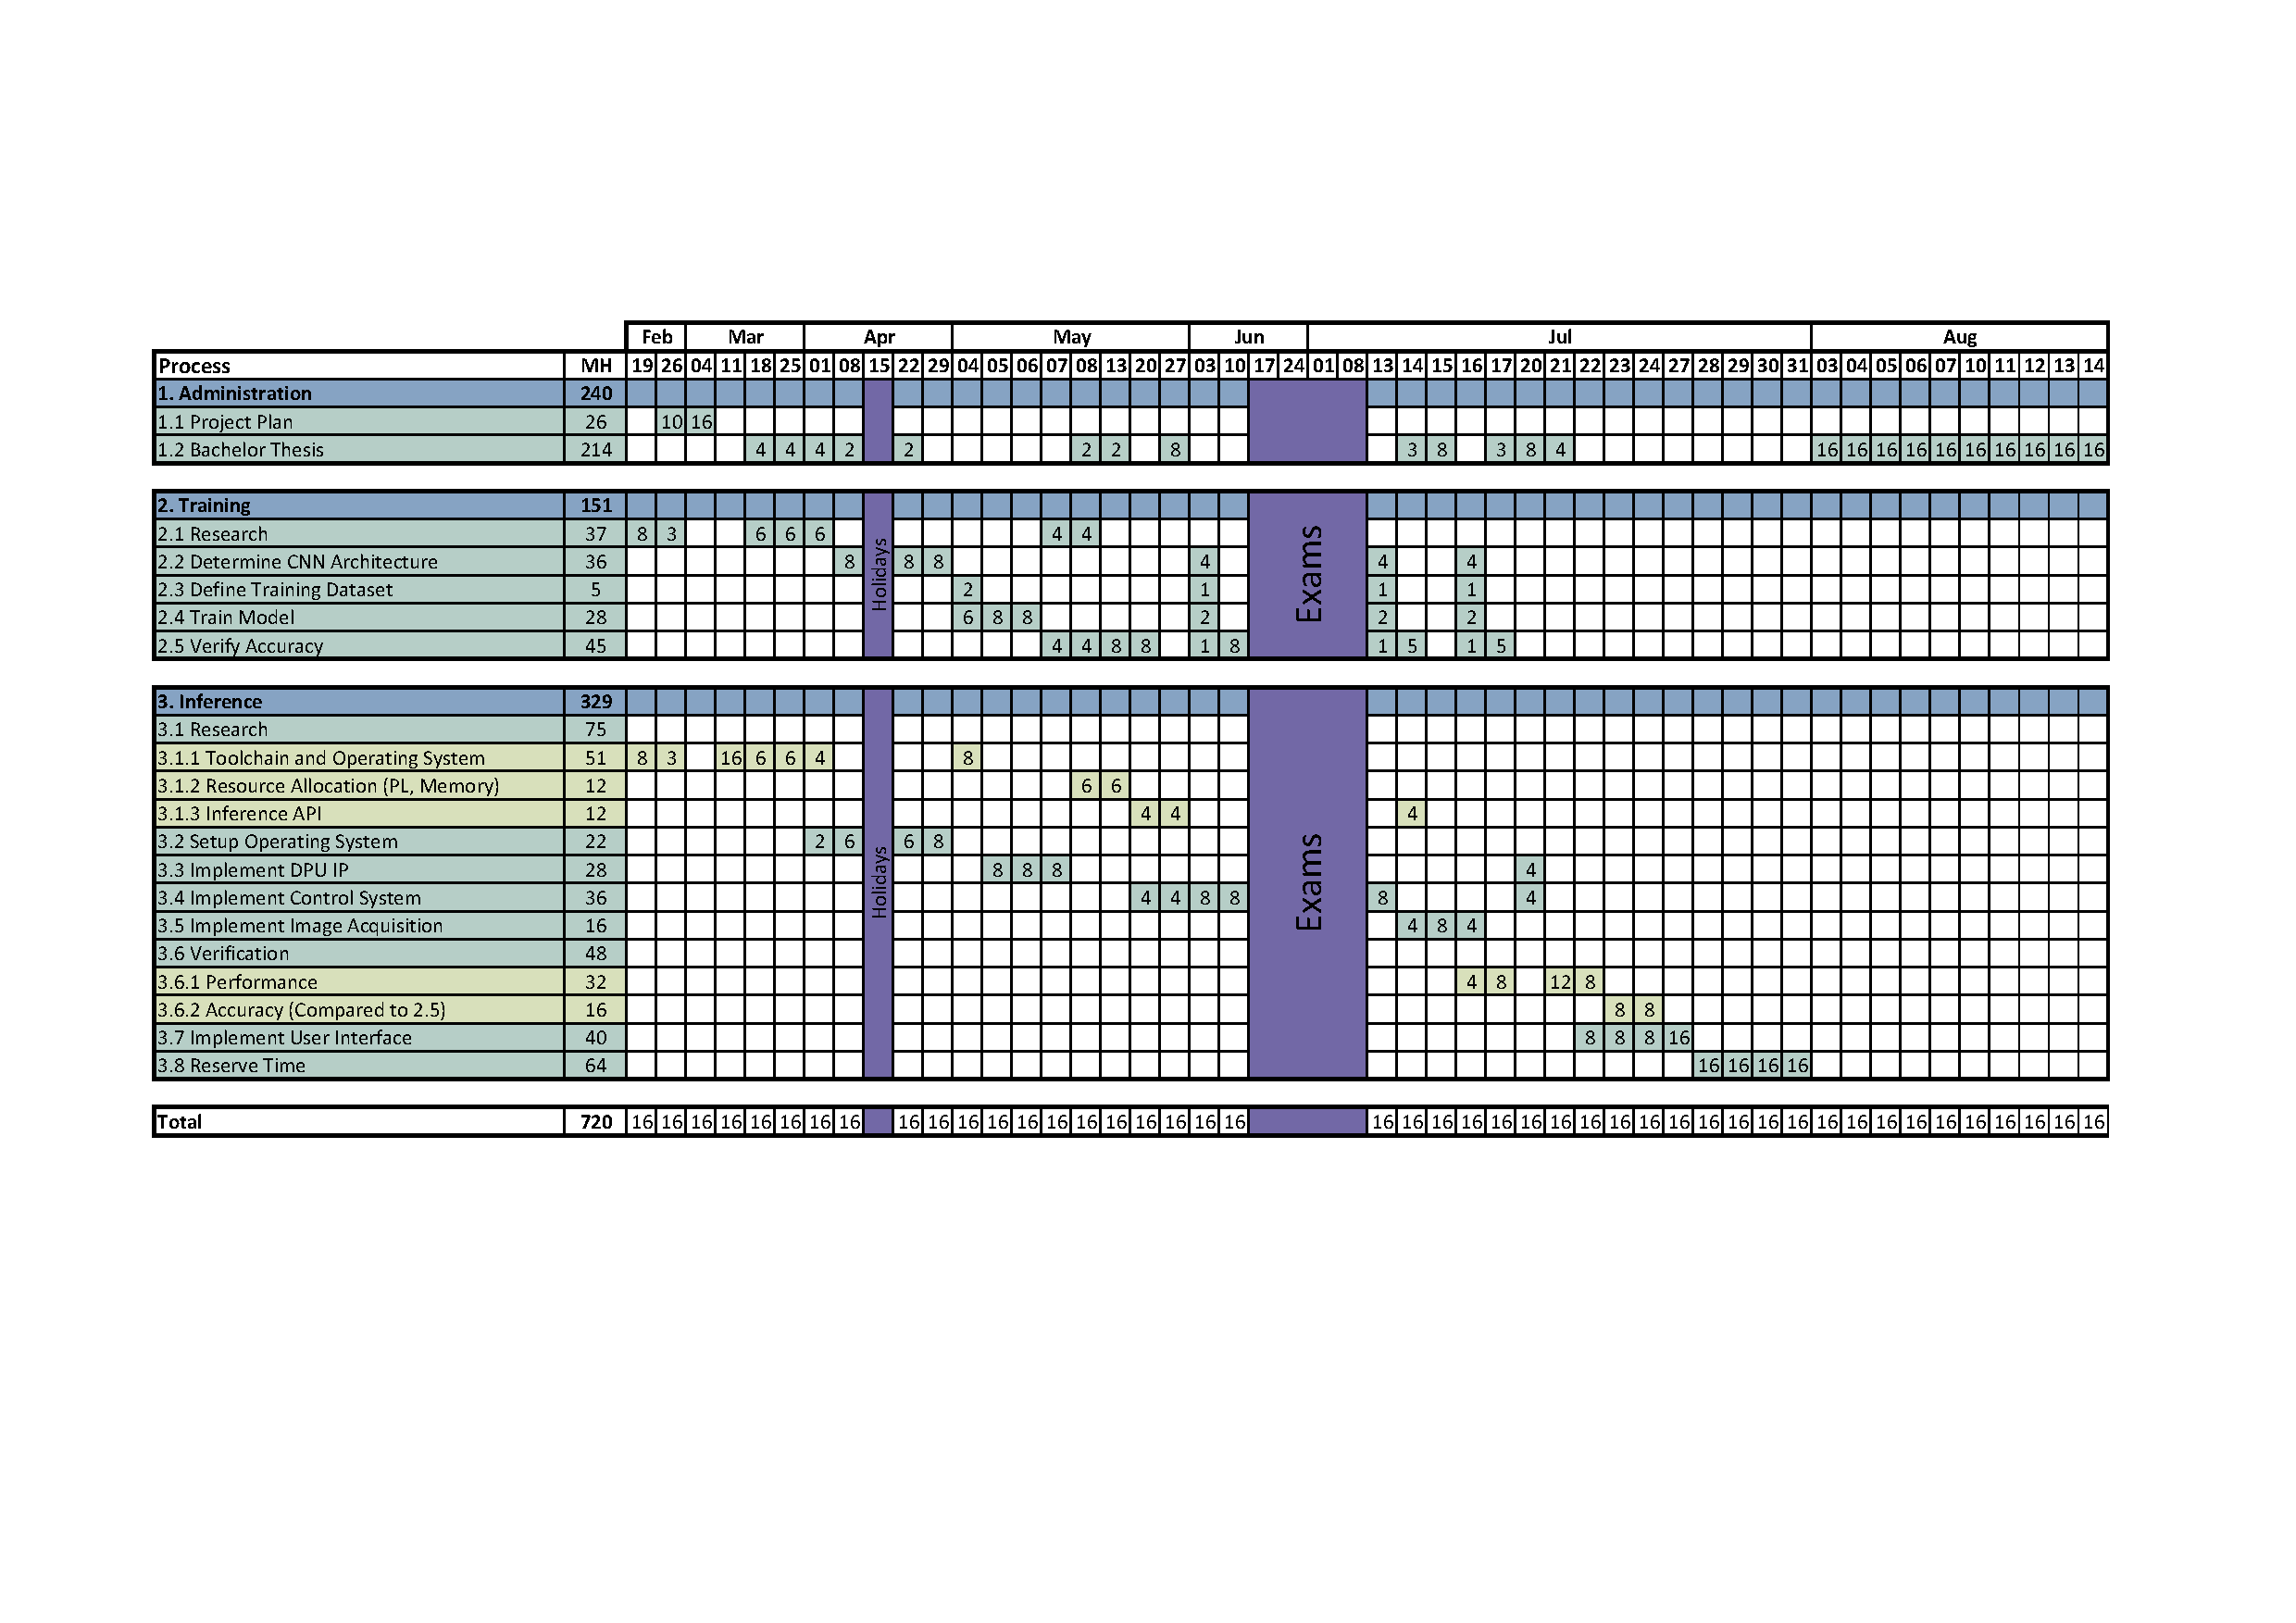
\includepdf[pages=-,landscape=true]{appendix/timetable.pdf}


% Bibliography
%\printbibliography[heading=bibintoc]
%\label{sec:literature}
%\clearpage

% Glossary
%\printglossaries
%\clearpage

% Appendix
\begin{appendix}
  \chapter{Problem Statement}
  \label{app:problem_statement}
  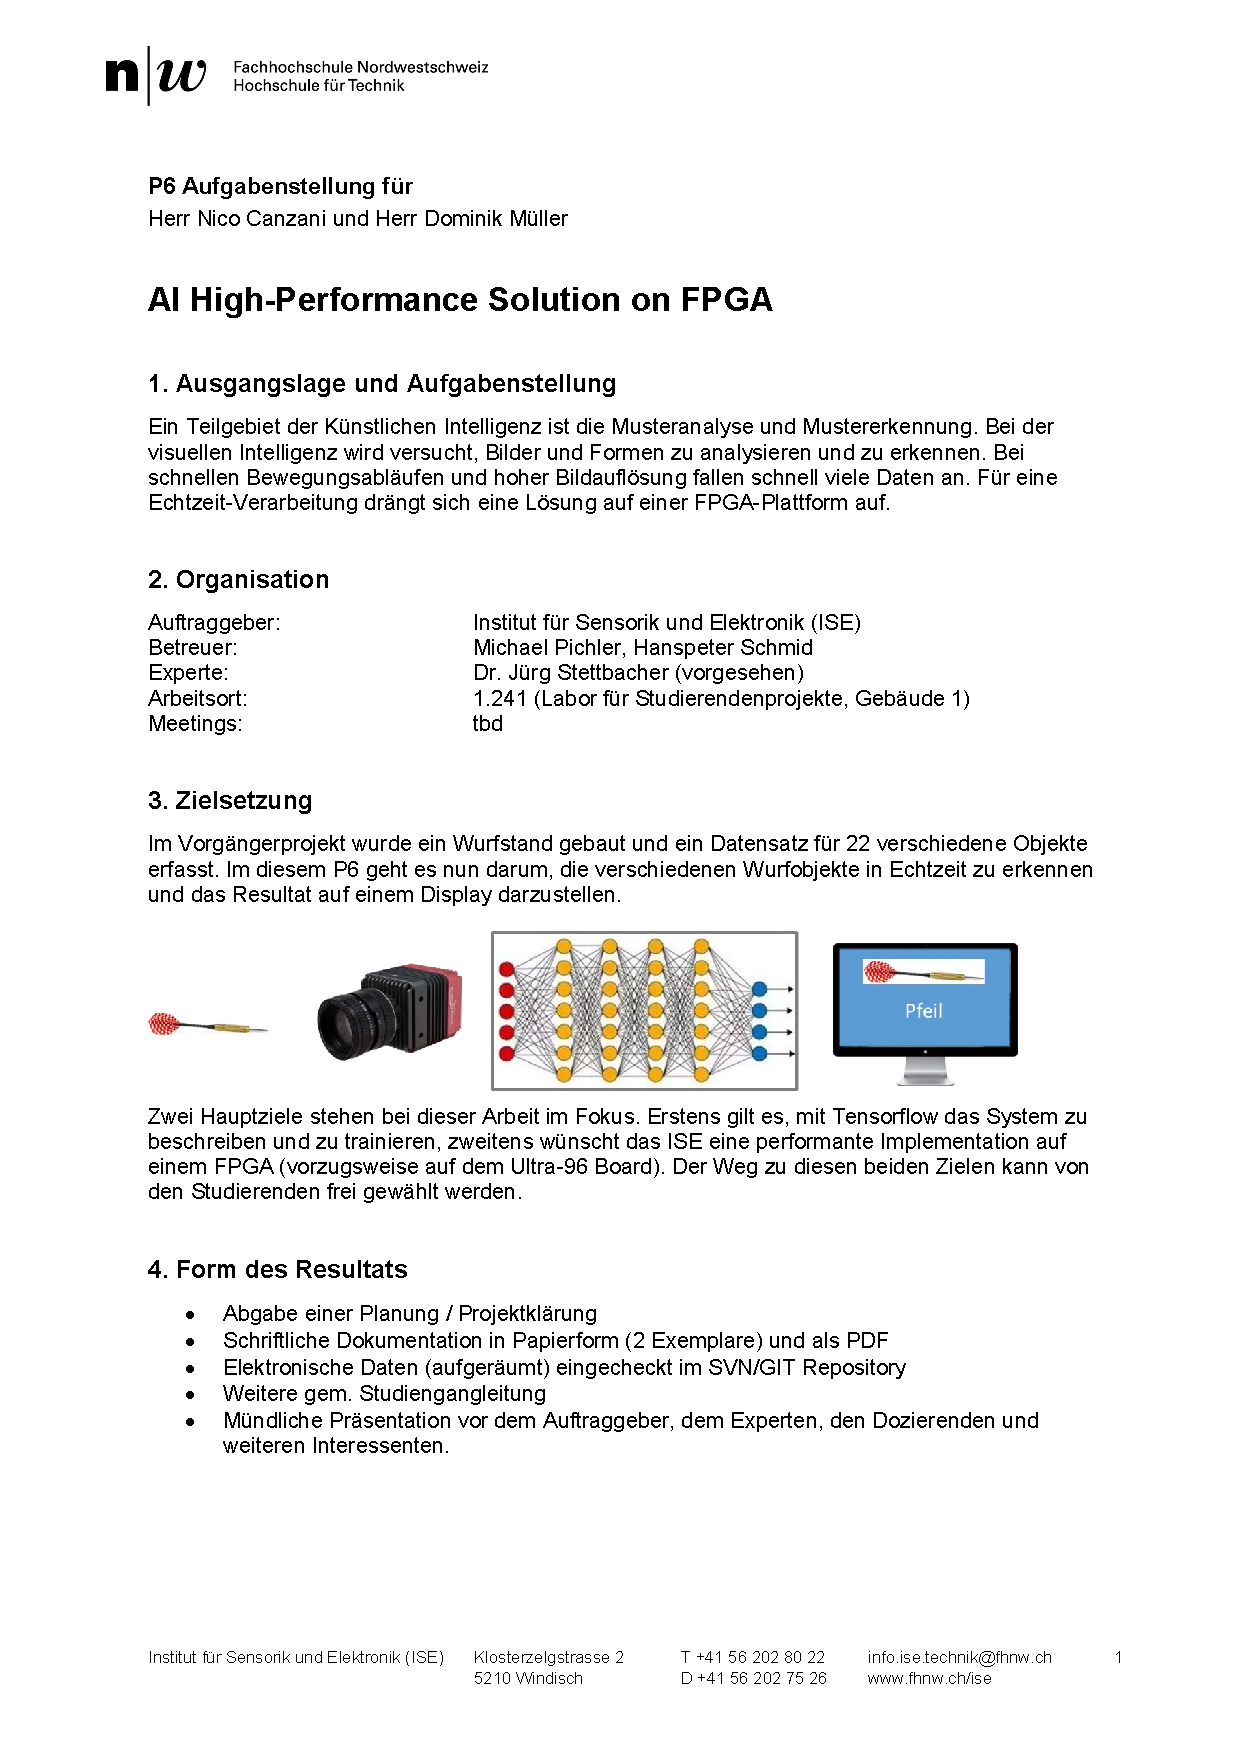
\includepdf[pages=-]{appendix/problem_statement.pdf}

  \chapter{Inference Application}
  \label{app:inference_application}
  \lstinputlisting[style=python]{appendix/aionfpga.py}
\end{appendix}


% Debug
%\newpage
%\listoftodos[\section{To-Do}]
%\clearpage

\end{document}
